\subsection{Design}
\label{norax:sec:design}

\point{NORAX Workflow}
\NORAX consists of four major components: \emph{
\NDisassembler,
\NPatcher,
\NLoader,
and \NMonitor}, as shown in Figure~\ref{fig:overview}. The first two components perform offline binary analysis and transformation and the last two provide runtime support for loading and monitoring the patched, XOM-compatible executables and libraries. 
%Given a  COTS binary, \NDisassembler disassembles and analyzes the binary. 
In addition to disassembling machine code, \NDisassembler scans for all executable code that needs to be protected by XOM. A major challenge it solves is identifying various types of data that ARM compilers often embed in the code section, including jump tables, literals, and padding. Unlike typical disassemblers, \NDisassembler has to precisely differentiate embedded data from code. 
%It collects all necessary information used by other components. 
Taking input from \NDisassembler, \NPatcher transforms the binary so that its embedded data are moved out of code sections and their references are collected for later adjustment. 
After the transformation, \NPatcher inserts a unique magic number in the binary so that it can be recognized by \NLoader during load-time. 
\NPatcher also stores \NORAX metadata in the binary, which will be used by \NLoader and \NMonitor. 
When a patched binary is being loaded, \NLoader takes over the loading process to (\rom{1}) load the \NORAX metadata into memory, (\rom{2}) adjust the \NPatcher-collected references as well as those dynamically created references to the linker-related sections (e.g .hash, .rela.*), and (\rom{3}) map all memory pages that contain code to XOM.
During runtime, 
%in several cases explained in the following section, 
\NMonitor, an OS extension, handles read accesses to XOM. While such accesses are rare and may indicate attacks, they could also be legitimate because \NPatcher may not be able to completely recognize dynamic references to the relocated embedded data (e.g., those generated at runtime). When there are missed data references, the access will trigger an XOM violation, which \NMonitor verifies and, if legitimate, facilitates the access to the corresponding data. 


\begin{figure*}[t]
\begin{center}
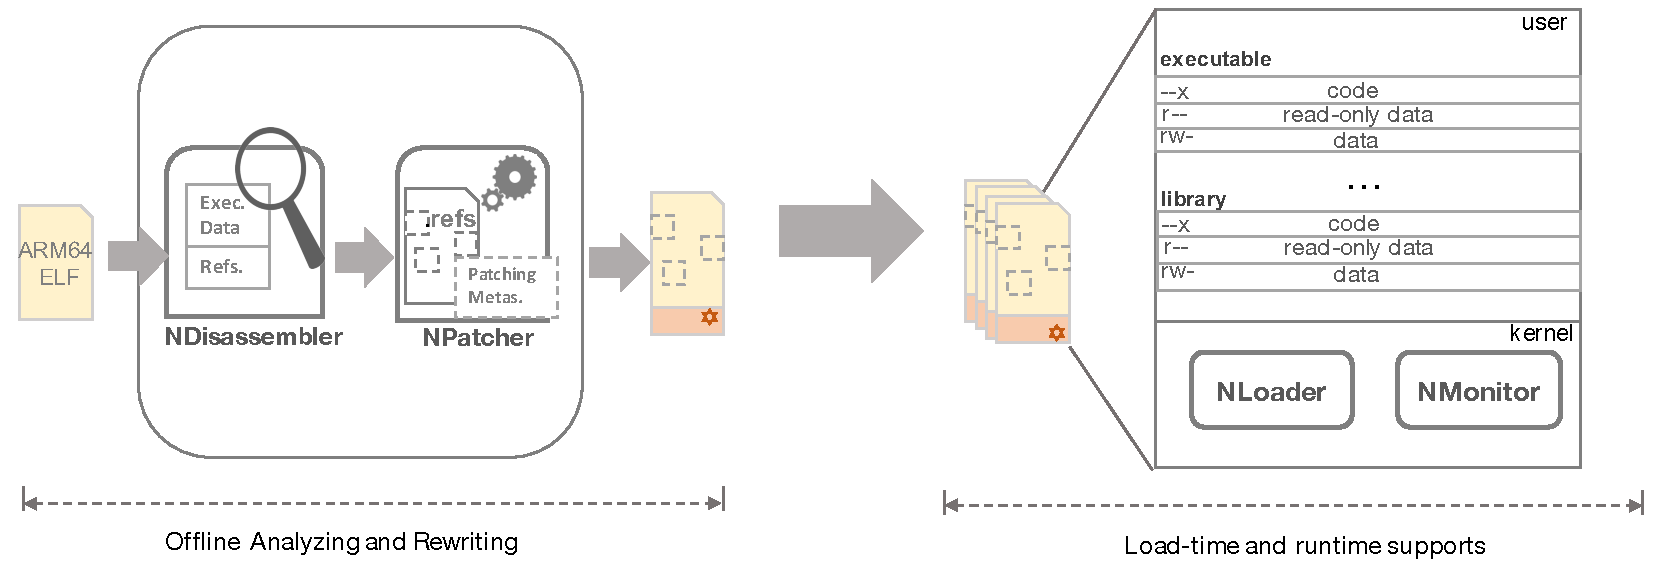
\includegraphics[scale=0.60]{norax/figures/overview}
\caption{NORAX System Overview: the offline tools (left) analyze the input binary, locate all the executable data and their references (when available), and then statically patch the metadata to the raw ELF; the runtime components (right) create separated mapping for the \emph{executable data sections} and update the recorded references as well as those generated at runtime.}
\label{fig:overview}
\end{center}
\end{figure*}


\subsubsection{\NDisassembler: Static Binary Analyzer}
\NDisassembler first converts an input binary from machine code to assembly code and then performs analysis needed for converting the binary into an XOM-compatible form. 
It disassembles the binary in a linear sweep fashion, which yields a larger code coverage than recursive disassembling \cite{linearsweep}. 

However, the larger code coverage comes at a 
cost of potentially mis-detecting embedded data as code (e.g., when such data happen to appear as syntactically correct instructions).
 \NDisassembler addresses this problem via an iterative data recognition technique. Along with this process, it also finds instructions that reference embedded data. 

The data recognition technique is inspired by the following observations:
\begin{itemize}
	\item Although it is difficult to find all instructions referencing some embedded data at a later point in the running program, it is relatively easy to locate the code that computes these references in the first place.
	\item To generate position-independent binaries, compilers can only use PC-relative addressing when emitting instructions that need to reference data inside binaries.
	\item AArch64 ISA only provides two classes of instructions for obtaining PC-relative values, namely the {\tt ldr (literal)} instructions and {\tt adr(p)} instructions.
\end{itemize}

\NDisassembler uses Algorithm~\ref{algo:seedcollection} to construct an initial set of embedded data (IS) and a set of reference sites (RS).
%to them as well as to \textit{.rodata} section. 
For embedded data whose size cannot be precisely bounded, \NDisassembler collects their seed addresses (AS) for further processing.
%As shown in Line 3 and Line 4--16 in Algorithm~\ref{algo:seedcollection}, \NDisassembler finds and adds two types of embedded data to IS: (\rom{1}) invalid instructions 
%(ie., cannot be disassembled), which are certainly embedded data because in AArch64 all instructions are aligned and of a fixed-size; 
%(\rom{2}) bytes (in \textit{.text} section) used by memory-load instructions. 
As shown in Line 5--9 in Algorithm~\ref{algo:seedcollection}, since the load size for {\tt ldr-literal} instructions is known, the identified embedded data are added to 
IS. On the other hand, the handling for {\tt adr} instructions is more involved, as shown in Line 10--27. \NDisassembler first performs forward slicing on {\tt xn} --- 
the register which holds the embedded data address. All instructions that have data dependencies on {\tt xn} are sliced, and {\tt xn} is considered {\em escaped} if 
any of its data-dependent registers is either (\rom{1}) stored to memory or (\rom{2}) passed to another function before being killed. In either case, the slicing also stops. If not all memory
dereferences based on {\tt xn} can be identified due to reference escaping, the size of the embedded data cannot be determined. Therefore, \NDisassembler only adds the initial value of {\tt xn} to 
AS, as a seed address (Line 24--26).

Line 10--23 of Algorithm~\ref{algo:seedcollection} deal with the sliced instructions. If a memory load based on {\tt xn} is found, RS is updated with the location of the original
address-taking instruction. Moreover, \NDisassembler analyzes the address range for each memory load. Note that oftentimes the address range is bounded because embedded data are mostly integer/floating point constants, or jump tables. In the former case, the start address of memory load is typically {\tt xn} plus some constant offset, while the load size is explicit from the memory load instruction. In the latter, well-known techniques for determining jump table size \cite{jump-table-analysis} are utilized. 
%Specifically, the address for accessed jump table entry is first computed as an expression
%such as $table\_base + 4 * index$, since $table\_base$ is a constant known from code and $index$ can be 
%bounded based on a comparison instruction between a register and a constant, the address range for the jump
%table can be determined.
In both cases, the identified embedded data are added into IS. However, if there is a single memory load whose address range cannot be bounded, \NDisassembler adds the seed address to AS. 

%The second case is necessary since there could be spurious instructions that are actually data but happen to be decodable. 
%This is common in stripped binaries where function boundary information is unknown. 
%Listing~\ref{list:spurious} shows one such example in Bionic Libc. 
%For \textit{.rodata} references it is similar to the routine shown in Algorithm~\ref{algo:seedcollection}, except that for cross-section references, due to the limited maximum addressing range $adr$ instruction could have, instead $adrp$ is used to perform the PC-relative references. 




\begin{figure*}[t]
	\centering
	\begin{minipage}[b]{0.45\textwidth}
		\centering	
		\begin{algorithm}[H]
		\caption{Initial embedded data and references collection}
		\label{algo:seedcollection}
		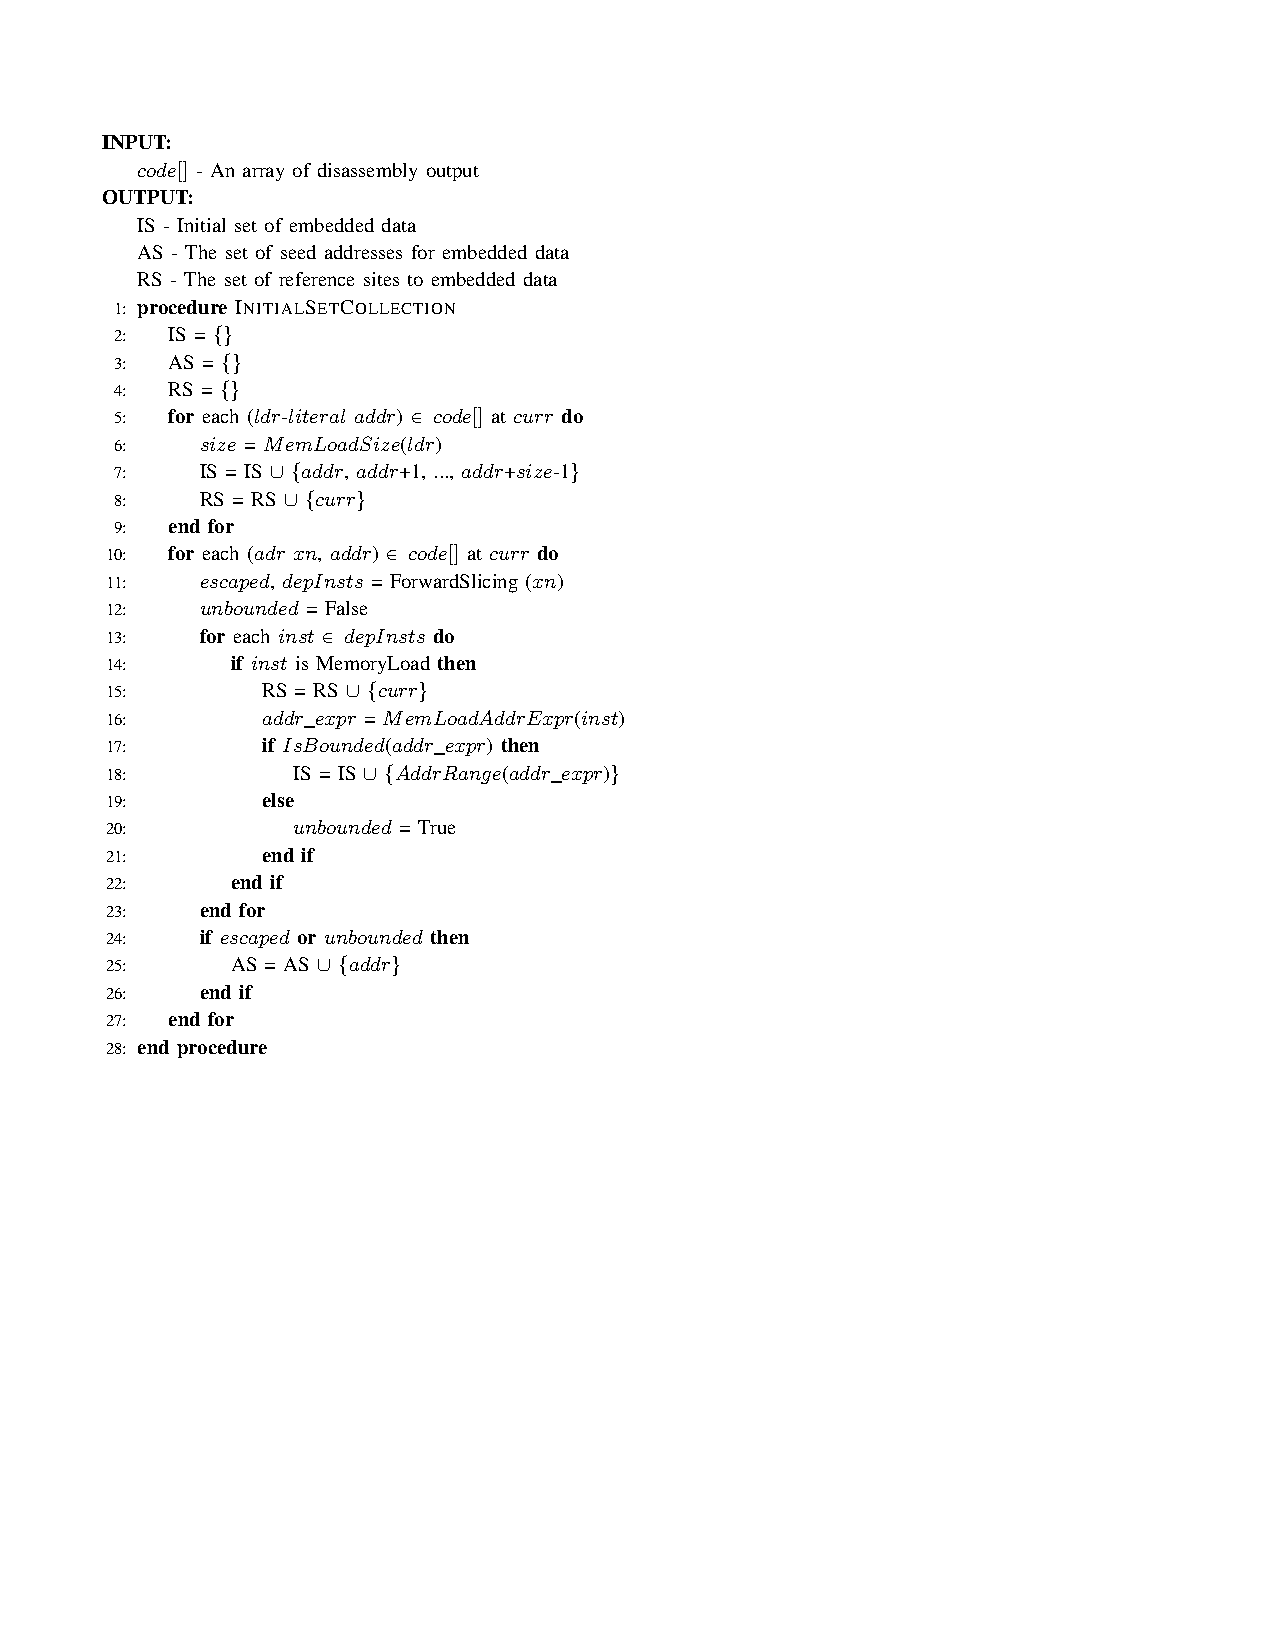
\includegraphics[width=\textwidth]{norax/figures/datarefcollection}
		\end{algorithm}
	\end{minipage}
 	\hfill
	\begin{minipage}[b]{0.45\textwidth}
		\centering	
		\begin{algorithm}[H]
		\caption{embedded data set expansion}
		\label{algo:seedexpansion}
		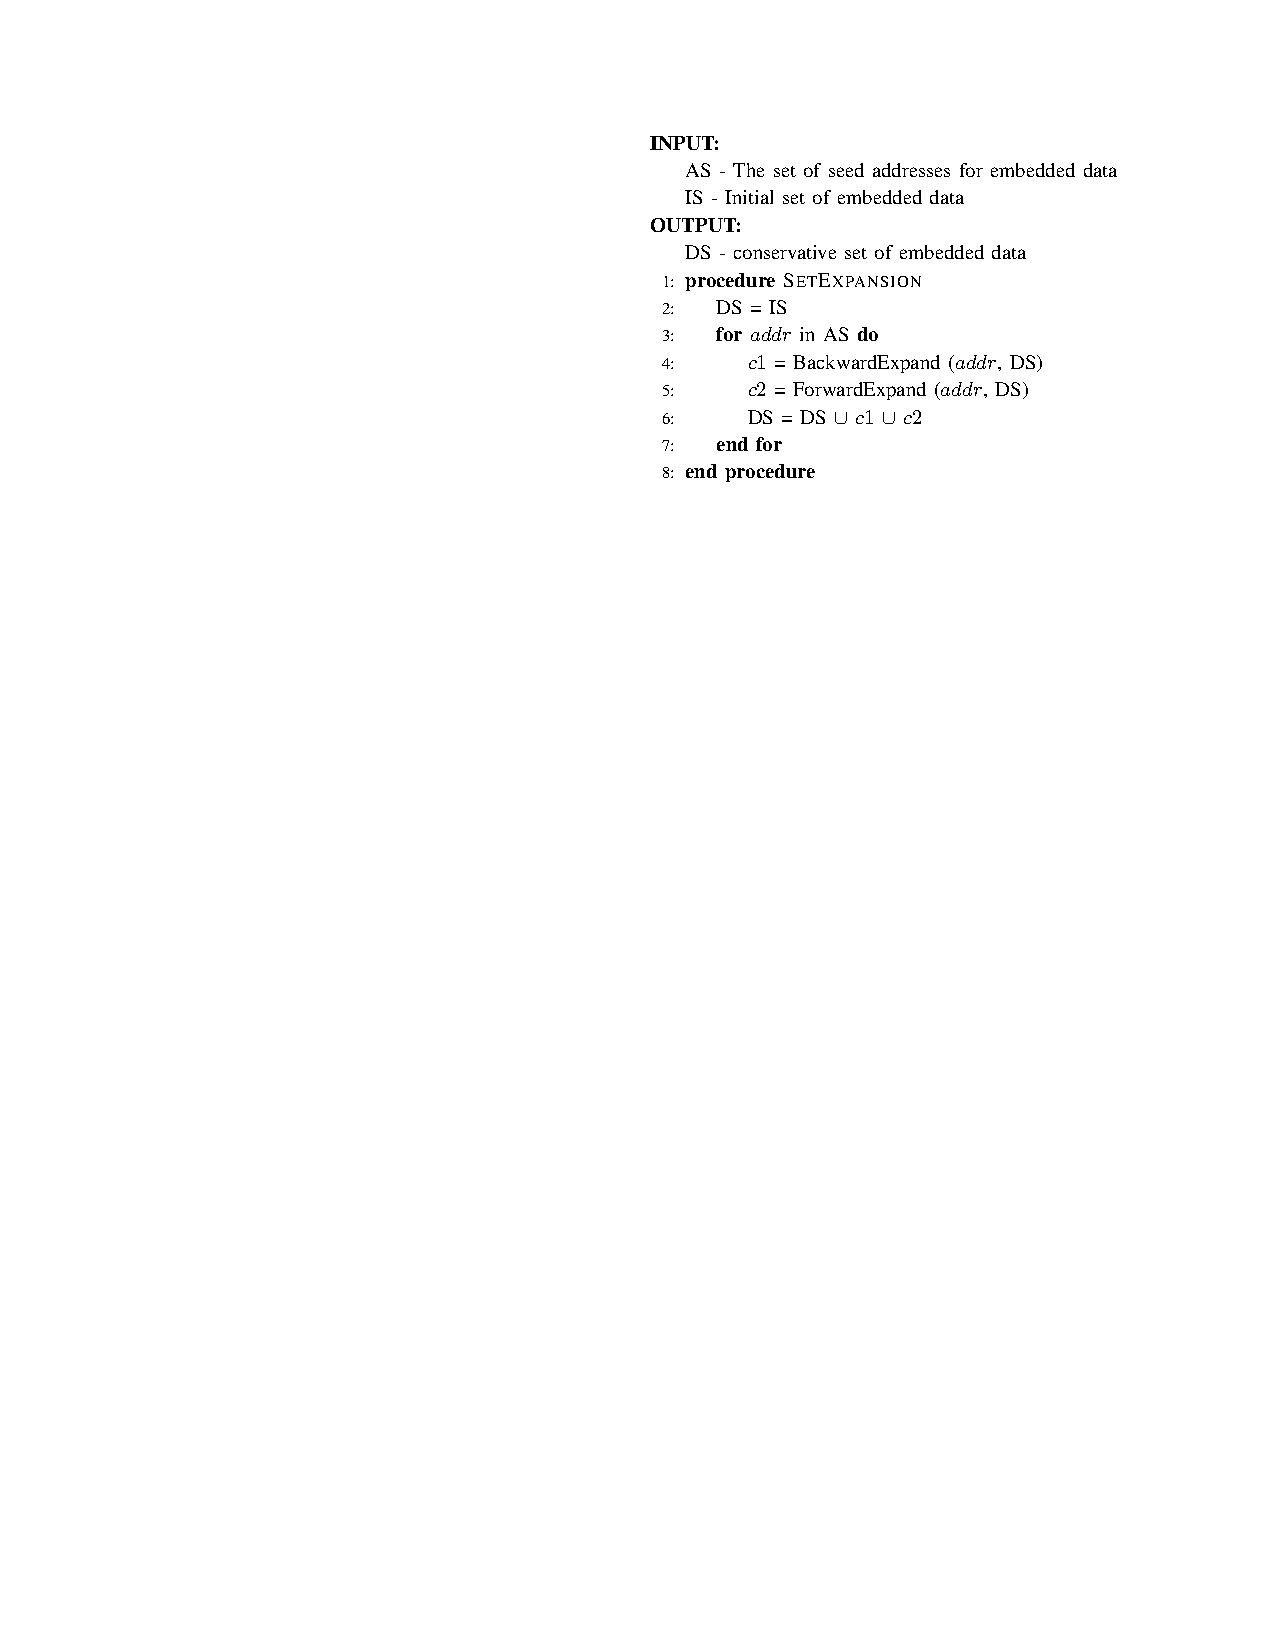
\includegraphics[width=\textwidth]{norax/figures/datasetexpansion}
		\end{algorithm}	
	\end{minipage}
\end{figure*}


%\begin{minipage}[t]{0.45\textwidth}
%\centering
%\begin{algorithm}[H]
%\caption{Initial embedded data and references collection}
%\label{algo:seedcollection}
%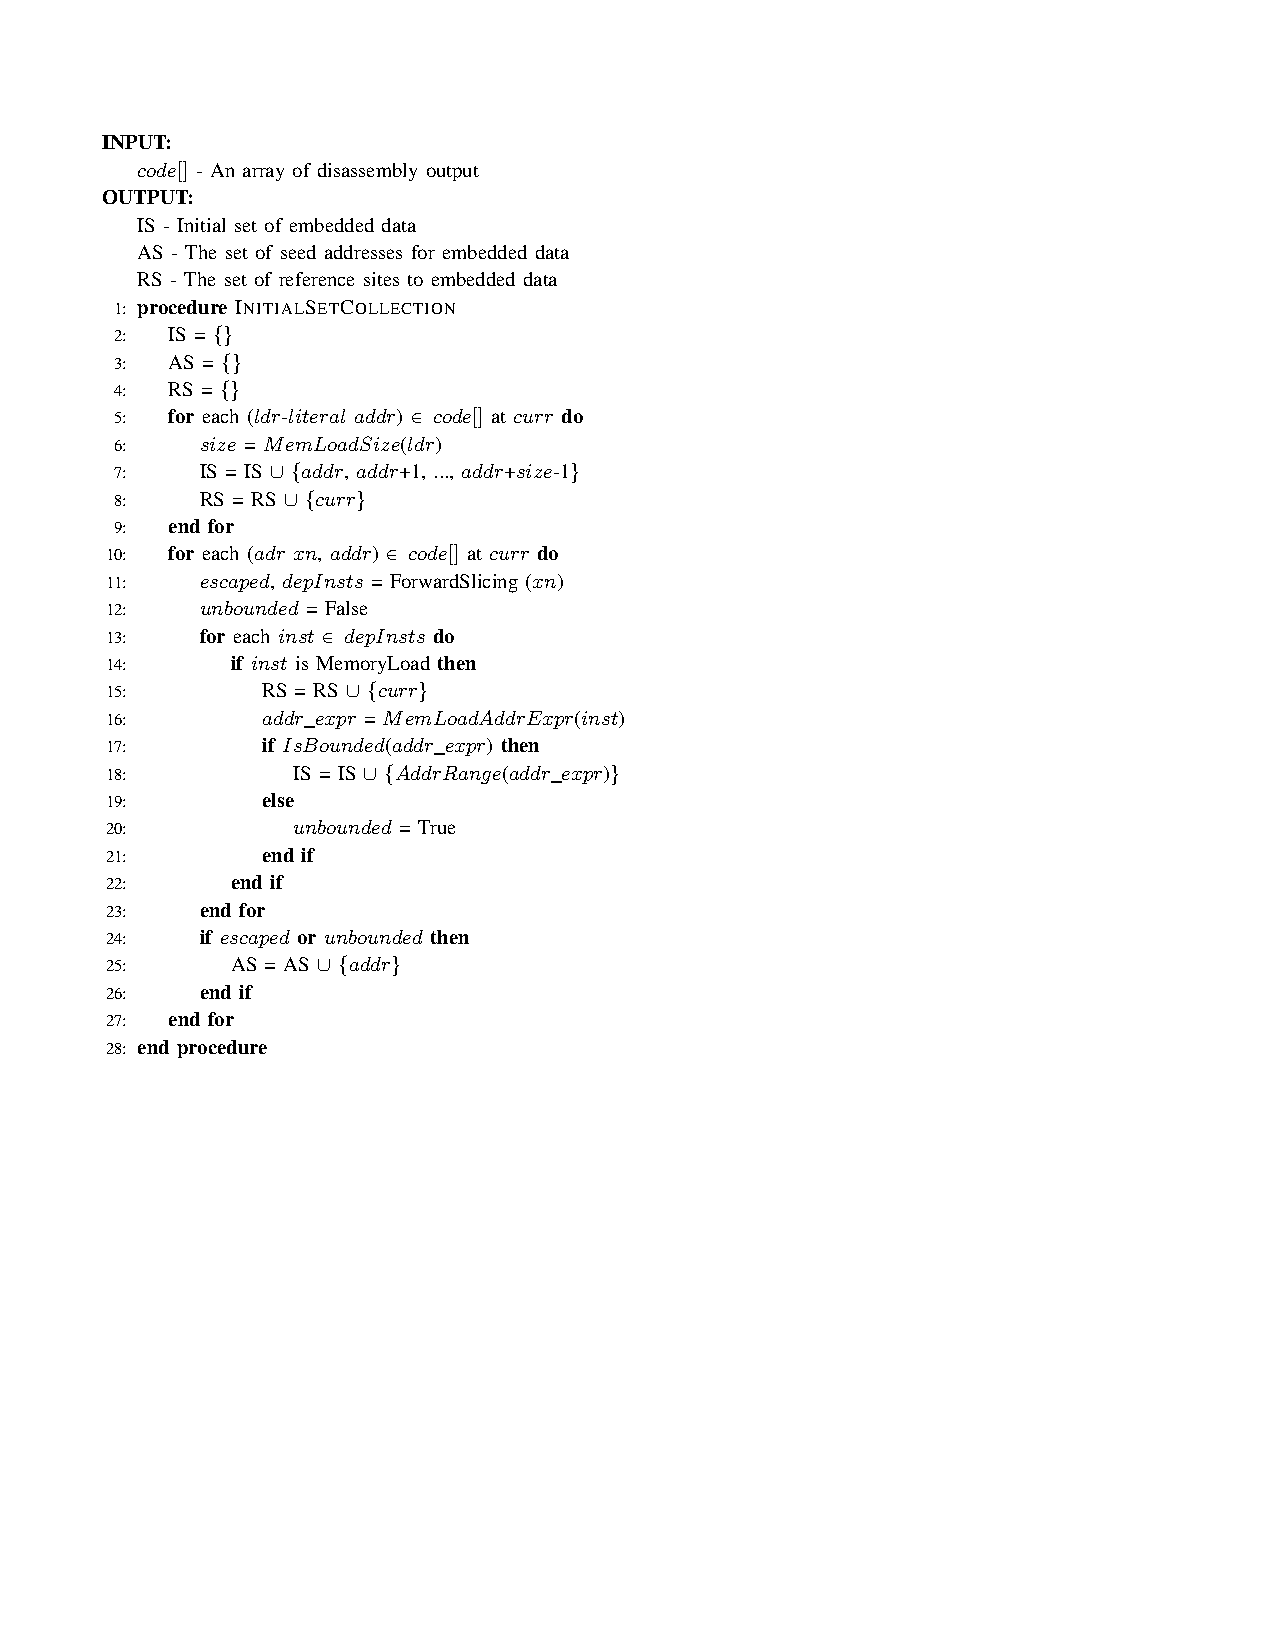
\includegraphics{norax/figures/datarefcollection}
%\end{algorithm}
%\end{minipage}
% 
%\begin{minipage}[t]{0.45\textwidth}
%\centering
%\begin{algorithm}[H]
%\caption{embedded data set expansion}
%\label{algo:seedexpansion}
%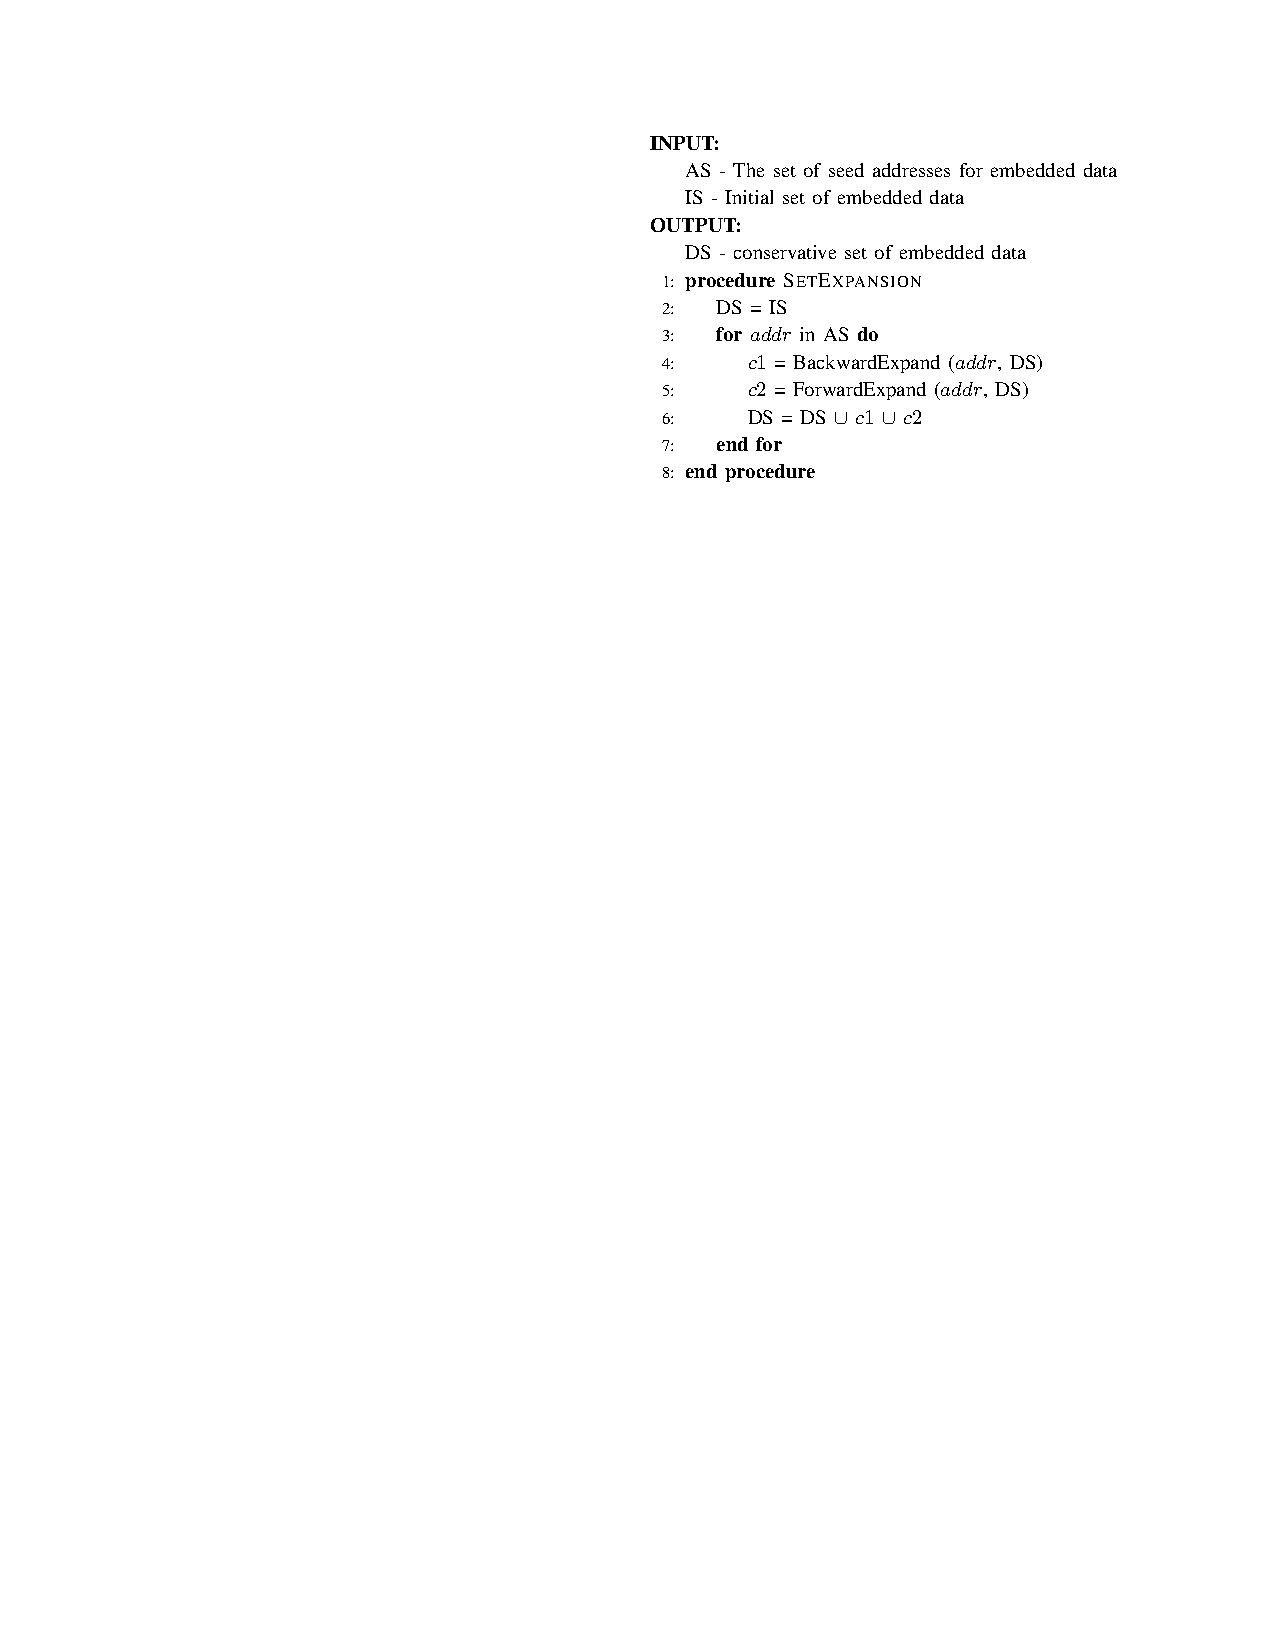
\includegraphics{norax/figures/datasetexpansion}
%\end{algorithm}
%
%\end{minipage}



%
%\begin{algorithm}[!t]
%\caption{Initial embedded data and references collection}
%\label{algo:seedcollection}
%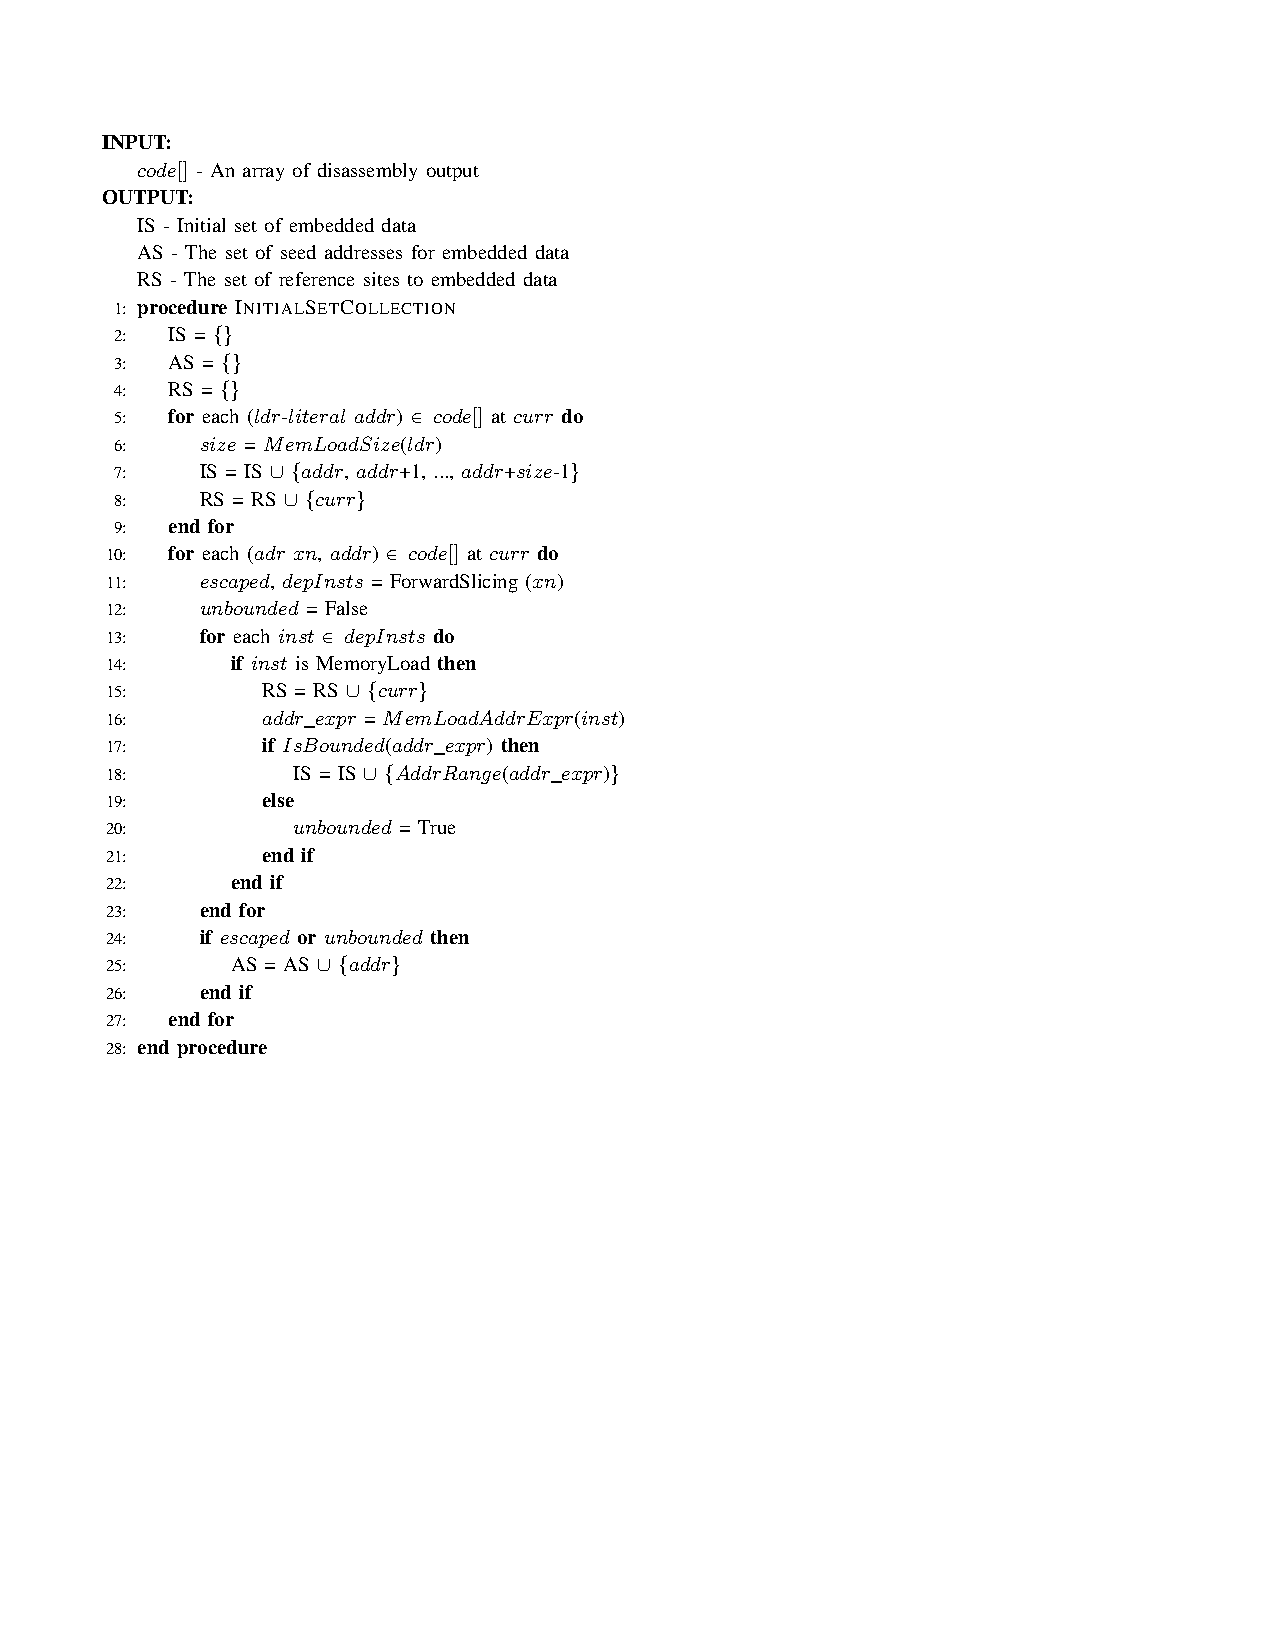
\includegraphics{norax/figures/datarefcollection}
%\end{algorithm}
%
%
%\begin{algorithm}[!t]
%\caption{embedded data set expansion}
%\label{algo:seedexpansion}
%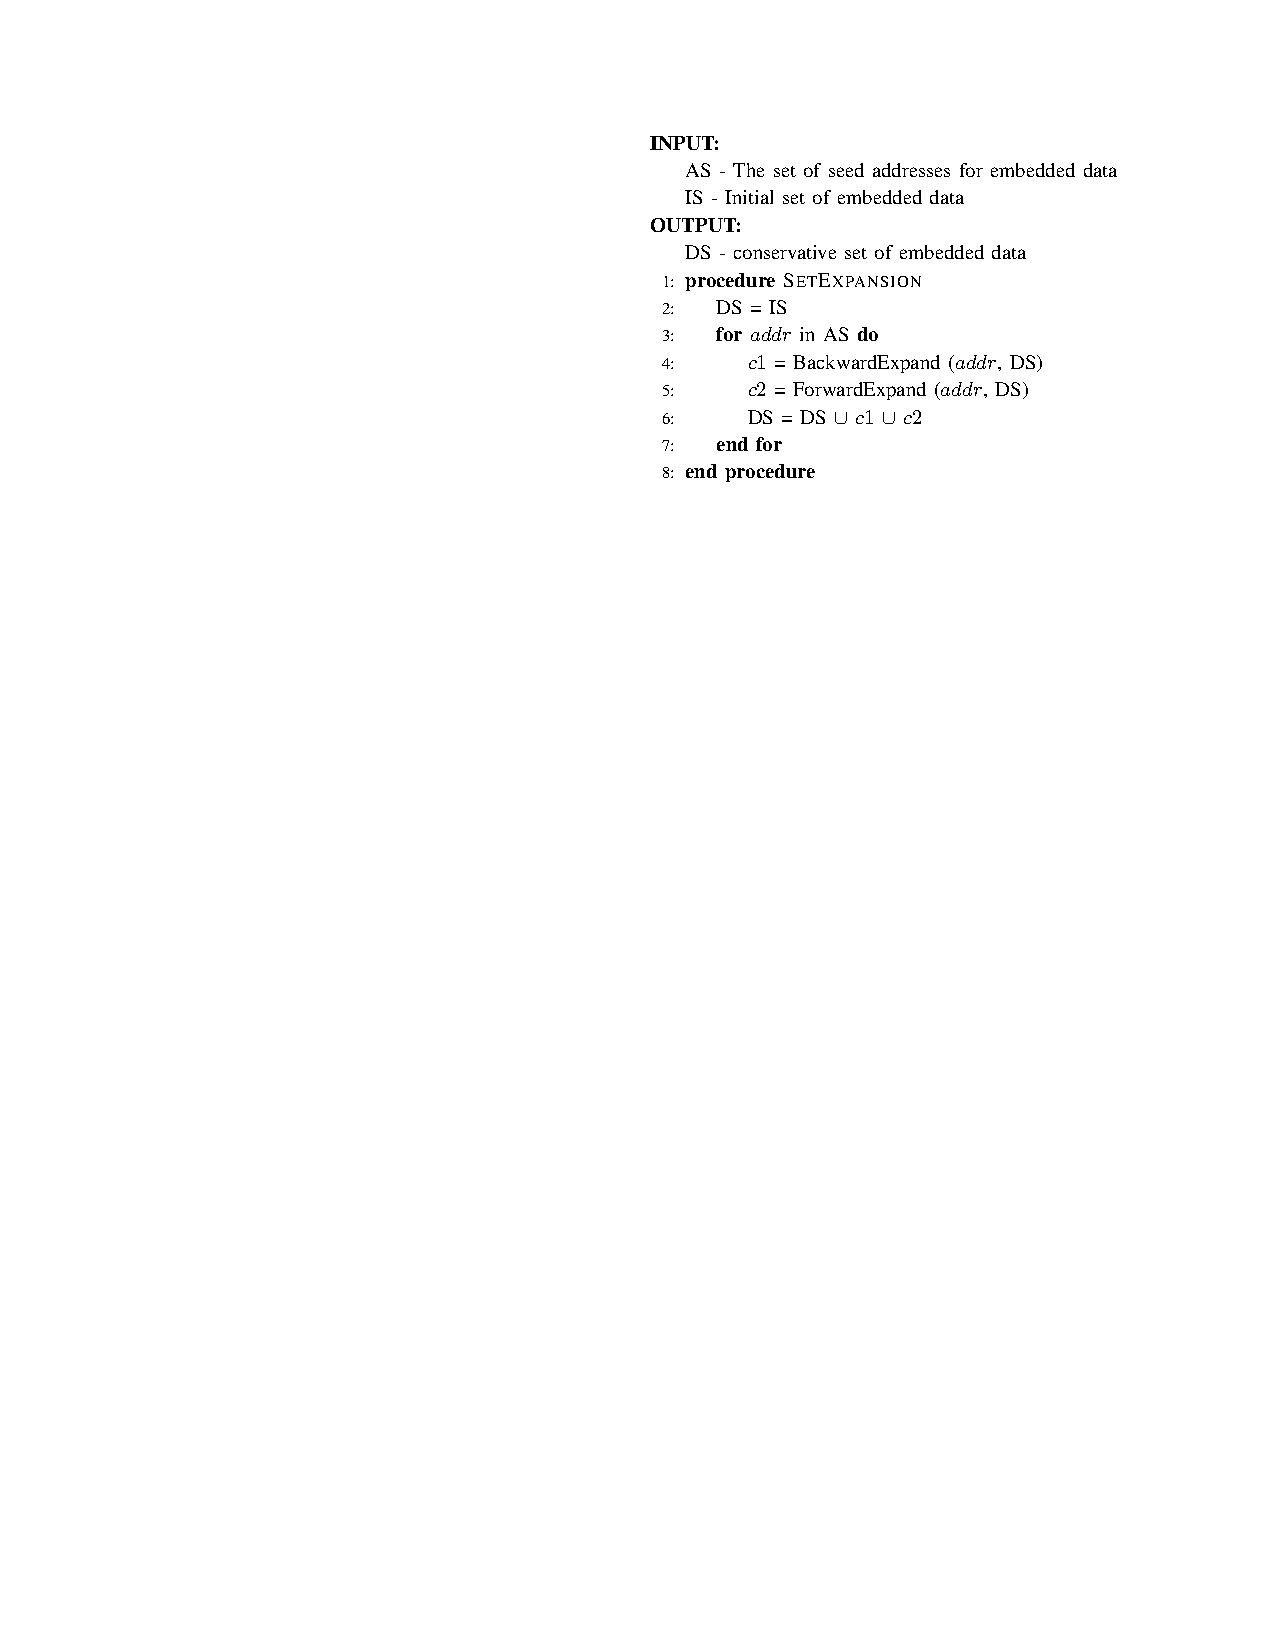
\includegraphics{norax/figures/datasetexpansion}
%\end{algorithm}

If Algorithm~\ref{algo:seedcollection} is not able to determine the sizes of all embedded data, the initial set (IS) is not complete. In this case,
the seed addresses in AS are expanded using Algorithm~\ref{algo:seedexpansion} to construct an over-approximated set of embedded data (DS). The core 
functions are $BackwardExpand$ (line 4) and $ForwardExpand$ (line 5). The backward expansion starts from a seed address and walks backward from that address until it encounters a \emph{valid} control-flow transfer instruction: i.e., the instruction is 
either a \emph{direct} control-flow transfer to a 4-byte aligned address in the address space, or an \emph{indirect} control-flow transfer.
%a direct control-flow transfer to a 4-byte aligned address in the address space.
All bytes walked through are marked as data and added to DS. 
On the other hand, the forward expansion 
% starts from the last instruction in the first basic block that immediately follows the embedded data. 
walks forward from the seed address. It proceeds aggressively for a conservative inclusion of all embedded data. It only stops when it has strong indication that it has identified a valid code instruction. These indicators are one of the following: (\rom{1}) a \emph{valid} control-flow transfer instruction is encountered, (\rom{2}) a direct control-flow transfer target (originating from other locations) is reached, and (\rom{3}) an instruction is confirmed as the start of a function\cite{fia}.  In the last case, comprehensive control-flow and data-flow properties such as parameter passing and callee saves are checked before validating an instruction as the start of a function. 
%After all expanded data are determined and added to DS, the initial set (IS) of embedded data is also combined to form the final result.

Finally, DS contains nearly all embedded data that exists in the binary.
Although we could further leverage heuristics to include \emph{undecodable}
instructions as embedded data, it is not necessary because our conservative
algorithms already cover the vast majority (if not all) of them, and the
rest are mostly padding bytes which are never referenced. Theoretically,
failure to include certain \emph{referenced} embedded data could still happen
if a chunk of data can be coincidentally decoded as a sequence of instructions
that satisfies many code properties, but in our evaluation of \textit{over 300} stripped Android system binaries, we never encountered such a case.
RS contains a large subset of reference sites to the embedded data. Since
statically identifying all indirect or dynamic data references may not always
be possible, \NDisassembler leaves such cases to be handled by \NMonitor. 

\subsubsection{\NPatcher: XOM Binary Patcher}
\point{Data Relocation}
%Given the analysis result that tells the locations of the executable data. \textit{Norax-tranz} needs to separate these data from their current positions so that they don't intermix with the real code. 
An intuitive design choice is to move the executable data out of the code segment. But doing so affects backward compatibility as the layout of the ELF and the offsets of its sections will change significantly. Another approach is to duplicate the executable data, but this would increase binary sizes and memory footprint significantly. 

Instead, \NPatcher uses two different strategies to relocate those executable data without modifying code sections or duplicating all read-only data sections. 
For data located in code segment but are separated from code text (i.e., read-only data), \NPatcher does not duplicate them in binaries but only records their offsets as metadata, which will be used by \NLoader to map such data into read-only memory pages. 
For data mixed with code (i.e., embedded data), \NPatcher copies them into a newly created data section at the end of the binary. The rationale behind the two strategies is that read-only data usually accounts for a large portion of the binary size and duplicating it in binary is wasteful and unnecessary. On the other hand, embedded data is usually of a small size, and duplicating it in binaries does not cost much space. More importantly, this is necessary for security reasons. Without duplication, code surrounding data would have to be made readable, which reduces the effectiveness of XOM. 
%Also due to the absence of a perfect analysis for pin-pointing the references (\S~\ref{subsec:analyzer}), NPatcher chooses not to touch the executable data of the converting ELF while it's on disk, but prepares all necessary matadata for later \NPatcher to create
%It prepares the binary in a way that during load time, \NLoader can double-map embedded data in virtual memory by simply reading the metadata that \NPatcher stores in binary headers. 
% duplicate mapping for these data to different memory pages, so that when these duplicates are accessed, no access violations will be triggered. To prepare the binary for such mapping, NPatcher first copies the embedded data out based on the analysis result from \emph{Norax-ana}, it then creates a header with entries specifying the offsets of these executable data, as well as their expected virtual addresses.


%\emph{Norax-ana} only provides the references from \textit{.text} to D1 data, yet in the meantime majority of the references to D2 data come from outside of the operated ELF (loader and linker), thus these references are not updatable by NPatcher.  


%\point{Policy-based access verification}  
%To cope with the un-discovered D1 references and the external D2 references, NPatcher generates policies to assure their accesses can go through while potential abuses by attackers can not. The policy specifies that code from where could read which executable data. For example, the linker-use sections, such as \emph{.gnu.hash}, \emph{.dynsym}, \emph{.dynstr}, are access-able only to the code from the linker module. While for the \emph{.text} embedded data, different granularities are applicable, we could allow only code from the same module to have access or we could go more fine-grained, by allowing only code from the over-approximate hosting function to read them (Zhang et al \cite{bincfi} presented such algorithm to retrieve the conservative function boundaries). The key here is knowing the addresses of those executable data, which is available thanks to \emph{Noarx-ana}'s conservative analysis. 

\point{Data Reference Collections}
\NPatcher only collects the references from \textit{.text} to \textit{.text} (embedded data) and to \textit{.rodata} because they can be statically recognized and resolved. Other types of references are either from outside the module or statically unavailable, which are handled by \NLoader.


For references to embedded data, \NPatcher can directly include them based on \NDisassembler's analysis results.
% to locate what are the reference sites that need to be adjusted. 
But there is one caveat -- the instructions used to reference embedded data (i.e., \textit{adr} and \textit{ldr-literal}) have a short addressing range. Therefore, when we map their target data to different memory pages, it is possible that the instructions cannot address or reach 
% offset encoded in the reference instruction can not be large enough to reach
the relocated data. To solve this issue without breaking backward-compatibility, 
\NPatcher generates stub code to facilitate access to out-of-range data. The instructions of short addressing range are replaced with an unconditional branch instruction\footnote{\textit{ADR} can address +/- 1MB, while \textit{B(ranch)} can access +/- 128MB, which is far enough for regular binaries.}, which points to the corresponding stub entry. The stub code only contains unconditional load and branch instructions pointing to fixed immediate offsets. 
This design ensures that these stub entries cannot be used as ROP gadgets. 
%Their behaviors are deterministic thus cannot be controlled by the attacker, as they only read from deterministic data locations and branch back to fixed code addresses.

For references to the \textit{.rodata}, there is no addressing capability problem, because \textit{adrp} is used instead of \textit{adr}. However, a different issue arises. There are multiple sources from which such references could come. We identify 5 sources in our empirical study covering all Android system executables and libraries. \NPatcher can only prepare the locations of the first three offline while leaving the last two to be handled by \NLoader after relocations and symbol resolving are finish. 
\begin{itemize}
	\item \textbf{References from code (\textit{.text})}: 
these are usually caused by access to constant values and strings. 
%\emph{Norax-ana}'s analysis includes the locations of such references.
	\item \textbf{References from symbol table (\textit{.dynsym})}: 
when a symbol is located in \textit{.rodata}, there will be an entry in the symbol table, whose \textit{value} field contains the address of the exposed symbol. 
	\item \textbf{References from relocation table (\textit{.rela.dyn})}:
for a relocatable  symbol located in \textit{.rodata}, the relocation table entry's \textit{r\_addend} field will point to the symbol's address. 
	\item \textbf{References from global offset table (\textit{.got})}:
when a variable in \textit{.rodata} cannot be addressed due to the addressing limit(e.g., \textit{adrp} can only address +/- 4GB), an entry in the global offset table is used to address that far-away variable. 
	\item \textbf{References from read-only global data (\textit{.data.rel.ro})}: 
most binaries in Android disable lazy-binding. The \textit{.data.rel.ro} section contains the addresses of global constant data that need to be relocatable. After the dynamic linker finishes relocating them, this table will be marked as read-only, as opposed to the traditional \textit{.data} section.
\end{itemize}

Finally, the metadata (duplicates and references), the data-accessing stub code and the \NORAX header
%, and an identification magic number
are appended to the end of the original binary, as shown in Figure~\ref{fig:noraxelf}. Note that by appending the \NORAX-related data to the end of the binary, we allow patched binaries to be backward-compatible. This is because the ELF standard ignores anything that comes after the section header table. As a result, binaries transformed by \NPatcher can run on devices without \NORAX support installed. They can also be parsed and disassembled by standard ELF utilities such as \emph{readelf} and \emph{objdump}. Moreover, \NORAX-patched binaries are compatible with other binary-level security enhancement techniques.   


\begin{figure*}[t]
	\centering
	\begin{minipage}[b]{0.4\textwidth}
		\centering	
		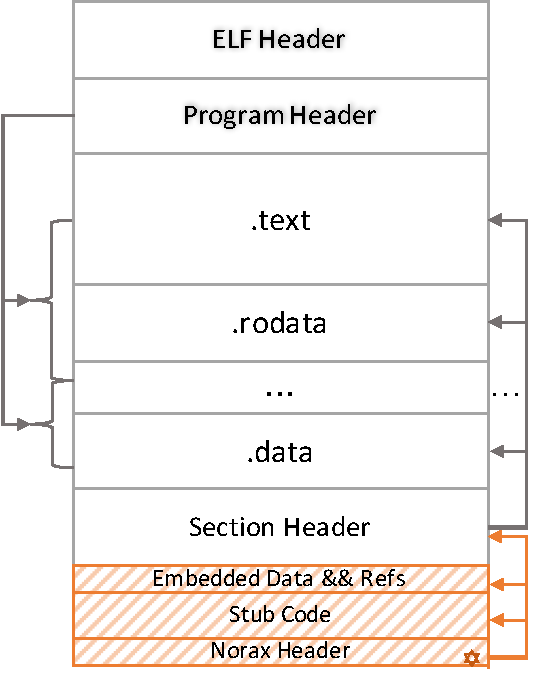
\includegraphics[scale=0.50]{norax/figures/norax-elf}
		\caption{The layout of ELF transformed by \NORAX. The shaded parts at the end are the generated \NORAX-related metadata.}
		\label{fig:noraxelf}
	\end{minipage}
 	\hfill
	\begin{minipage}[b]{0.5\textwidth}
		\centering	
		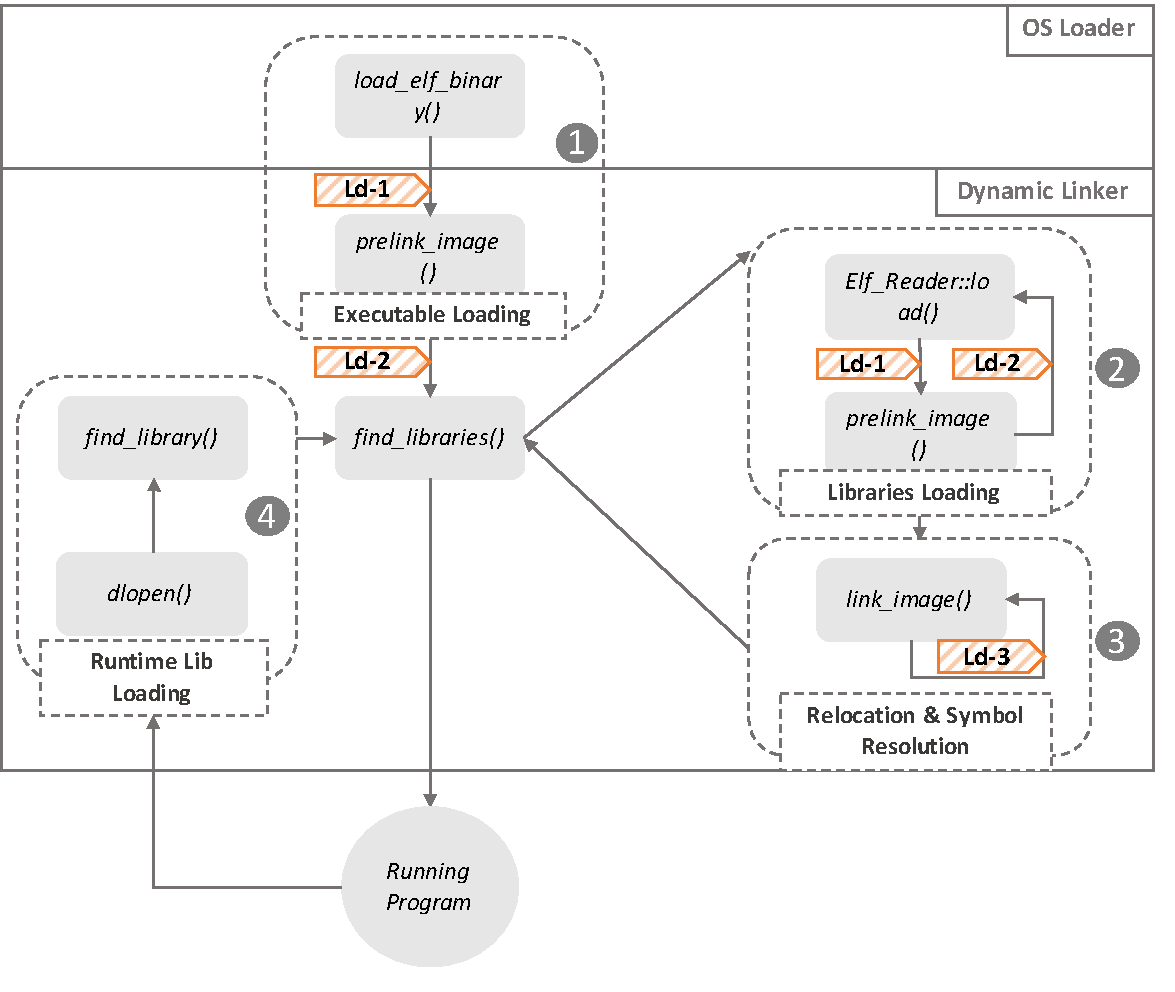
\includegraphics[scale=0.46]{norax/figures/norax-ldflow}
		\caption{Bionic Linker's binary loading flow, \NLoader operates in different binary preparing stages, including module loading, relocation and symbol resolution.}
		\label{fig:noraxld}
	\end{minipage}
\end{figure*}



%\begin{figure}[htb]
%\begin{center}
%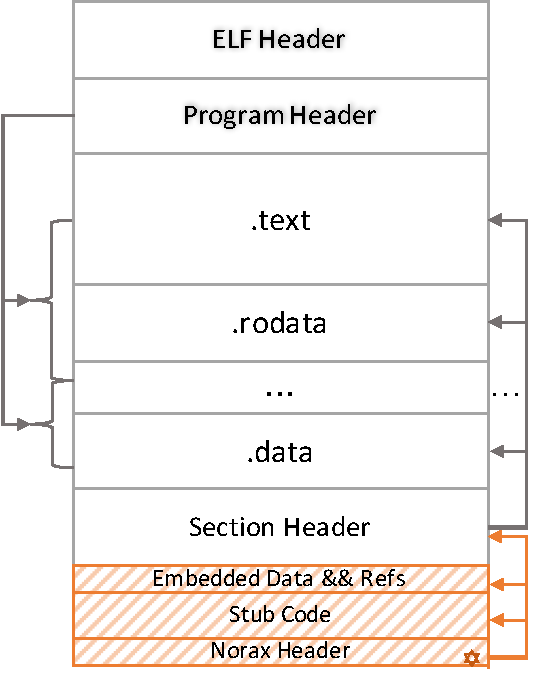
\includegraphics[scale=0.50]{norax/figures/norax-elf}
%\caption{The layout of ELF transformed by \NORAX. The shaded parts at the end are the generated \NORAX-related metadata.}
%\label{fig:noraxelf}
%\end{center}
%\end{figure}

\subsubsection{\NLoader: Plugin for Stock Loader and Linker}
\label{subsec:loader}
Binaries rewritten by NPatcher remain recognizable by and compatible with the stock loader and linker. They can still function albeit without the XOM protection. 
% as a result of NPatcher's careful elf-compatible binary transformation. 
New data sections added by \NORAX, however, are transparent to the toolchain. They require \NLoader's support to complete the binary loading and references updating process before their code can be mapped in XOM. 
Other than the ones prepared by \NPatcher, there are several types of references to executable data which are related to the linker and only available at runtime. Built as a linker/loader plugin, \NLoader adjusts these references in the following steps: 
%. In summary, three sub-tasks are performed by \NLoader during loadtime:
\begin{itemize}
	\item {\bf{Ld-1:}} It  parses and loads \NORAX header into memory, including information about the embedded data in \textit{.text} and the stub code accessing embedded data. Then, it creates duplicated mappings for \textit{.rodata} and the linker-referencing sections\footnote{The linker-referencing sections include \textit{.(gnu).hash, .dynsym, .dynstr, .gnu.version, .gnu.version\_r, .rela.dyn, .rela.plt}., etc.}, which have been loaded by the stock linker/loader.    
	\item {\bf{Ld-2:}} It updates the \textit{.dynamic} section to redirect linker to use the read-only copy of those relocated data sections.
	\item {\bf{Ld-3:}} It collects the \textit{.rodata} references from \textit{.got} and \textit{.data.rel.ro}, which are only populated after the relocation is done. It then adjusts all the collected data references in one pass. Eventually, the memory access level of the loaded module is adjusted to enforce the $\bf{R}\oplus\bf{X}$ policy.
\end{itemize} 

%\begin{figure}[ht]
%\begin{center}
%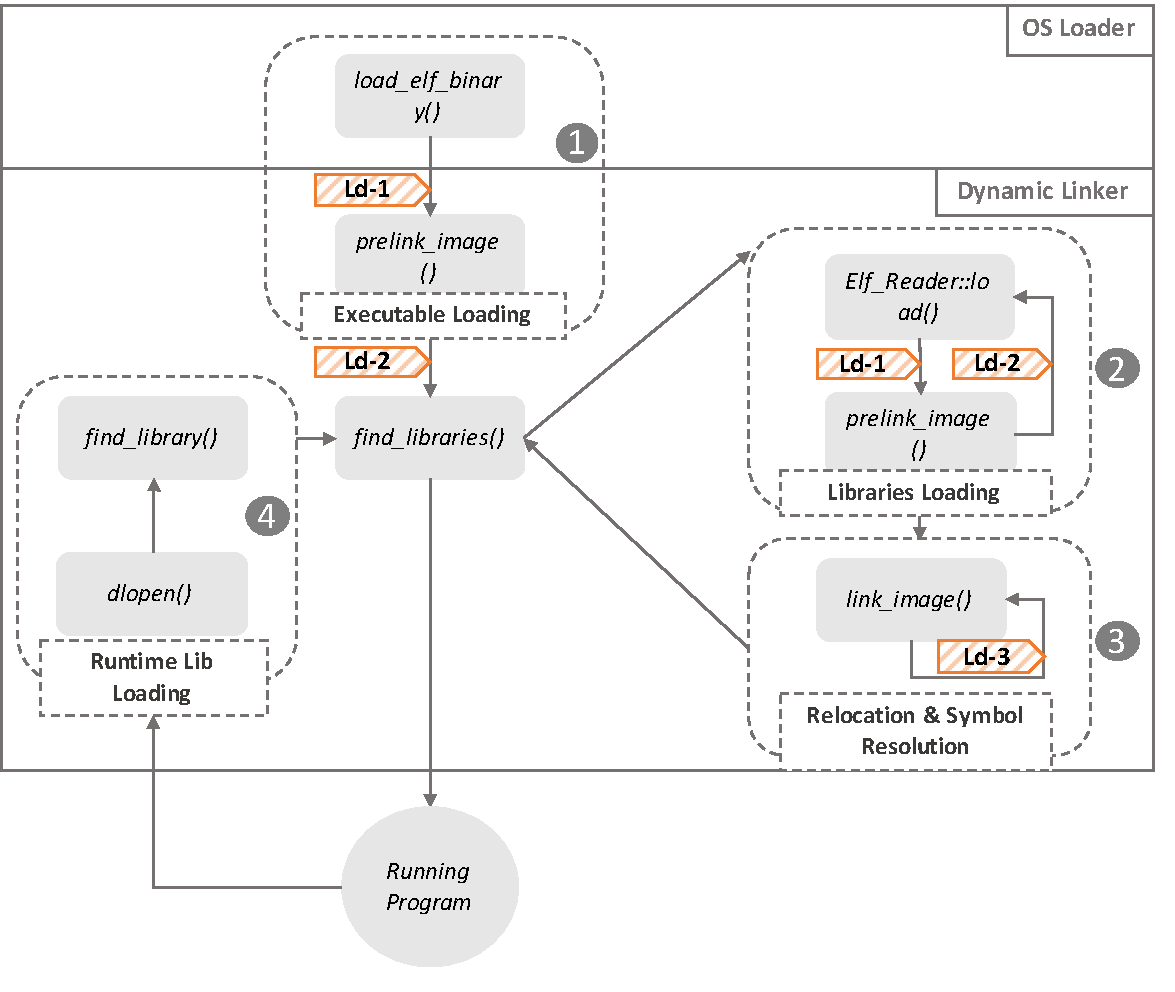
\includegraphics[scale=0.46]{norax/figures/norax-ldflow}
%\caption{Bionic Linker's binary loading flow, \NLoader operates in different binary preparing stages, including module loading, relocation and symbol resolution.}
%\label{fig:noraxld}
%\end{center}
%\end{figure}

The overall workflow of \NLoader is shown in Figure~\ref{fig:noraxld}. 
%The preparation of all the modules needed by a target program 
It starts with the executable loading, which is done by the OS ELF loader (Step \circled{1} ). 
Then, the OS loader transfers the control to the dynamic linker, which in turns creates a book-keeping object for the just-loaded module. Meanwhile, \textbf{Ld-1} is performed to complete the binary loading. Next, the binary's corresponding book-keeping object is then populated with references to those ELF sections used by the linker to carry out relocation and symbol resolution in a later stage. \textbf{Ld-2} is then invoked to update these populated references. 
At this point, the preparation for the executable is done. The linker then starts preparing all the libraries (Step \circled{2} ). This process is similar to the preparation of executable, thus \textbf{Ld-1} and \textbf{Ld-2} are called accordingly.  
%
When all the modules are loaded successfully in previous steps with their book-keeping objects populated, the linker walks through the book-keeping objects to perform relocation and symbol resolution (Step \circled{3} ). In this step, \textbf{Ld-3} is called for each of the relocated modules to update all those collected references, including the ones from \textit{.got} and \textit{.data.rel.ro} to \textit{.rodata}. This is feasible because the \textit{.got} entries which reference to \textit{.rodata} are populated upfront, same as those in \textit{.data.rel.ro}. 

During runtime, the program may dynamically load or unload new libraries (Step \circled{4} ), as shown in Figure~\ref{fig:noraxld}, which is also naturally handled by \NLoader. To boost performance, once \NLoader finishes updating the offline-updatable references, it caches the patched binary so that it can directly load the cached version without going through the whole references adjustment process again next time.

\subsubsection{\NMonitor: Runtime Enforcement and Safety-net}
After being processed by the last three \NORAX components, a patched binary that follows the $\bf{R}\oplus\bf{X}$ policy is ready to run, which is assisted by \NMonitor.
At runtime, the converted program could still be running with some unadjusted references to the executable data, which belong to the two following possible categories. 

\begin{itemize}
\item
{\bf Missed references to embedded data}:
Although in our evaluation we rarely see cases where an access violation is triggered by missed embedded data references, such situation, if mishandled, will cause a program crash. 
\NDisassembler is unable to discover such cases due to the limitation of static analysis.
These missed data references would trigger access violations. Note that references to \textit{.rodata} from \textit{.text} do not have this problem, because whenever an address is calculated that happens to point at \textit{.rodata} section, \NDisassembler will mark it as a valid reference regardless of whether a corresponding memory load instruction is detected or not. 
\item
{\bf References to \textit{.eh\_frame\_hdr} and \textit{.eh\_frame}}: 
These sections provide auxiliary information such as the address range of functions, the stack content when a C++ exception is triggered, etc. The previous components are unable to update them because they are used neither by the converted module itself nor by the dynamic linker. Instead, we found that C++ runtime and debuggers such as gdb would reference and read into these two sections for exception handling or stack unwinding.

\end{itemize}

\NMonitor dynamically handles both categories of unadjusted references. \NMonitor responds to memory violations caused by any attempted read access to XOM. It checks the context and the data being accessed. If the context matches the two cases discussed above and the address being accessed does belong to the relocated data, \NMonitor permits and facilitates the access; otherwise, it terminates the program. 
Specifically, \NMonitor whitelists these two kinds of data and ensures legitimate accesses to them can go through while potential abuses by attackers cannot. 
%The policy specifies that code from where could read which executable data. 
For instance, \NMonitor only allows C++ runtime module to access the \textit{.eh\_frame} sections (updatable through sysctl). 
For the \emph{.text} embedded data, \NMonitor only allows code from the over-approximated hosting function to read them.
Note that while this design helps our system cope with those corner cases, the security of our system is barely undermined for two reasons: (\rom{1})  the majority of the whitelisted data are indeed \emph{real} data, which are not even decodable or surrounded by non-decodable data. (\rom{2}) Different data require code from different regions to access them; attackers cannot simply exploit one memory leak bug to read across all these embedded data. 
